\section{Data Collection}
\label{sec:int}

The task of noun phrase linking is more difficult than \nel{}, due to the difficulty of finding indirect links.  Because of this, we develop methods to efficiently collect data.
The Quizzical Entity Linking (\quel{}) dataset is annotated with an interface (Figure~\ref{fig:nel-int}) that supports basic entity linking functionality (Section~\ref{sec:el-int}), configurable inclusion of machine-generated links to vary annotation conditions, and features to motivate expert annotators to participate in data collection (Section~\ref{sec:packet}).
Gold data will be collected by the authors of this paper (Section~\ref{sec:gold}), and all other data will be collected by organizers of \qb{} tournaments (Section~\ref{sec:expert}).
We plan to utilize human-in-the-loop annotation to help annotators and speed up the annotation process (Section~\ref{sec:active}) and assist users by pre-linking certain entities (Section~\ref{sec:other-ent}). 

\subsection{Entity Linking Interface}
\label{sec:el-int}

To collect the \quel{} dataset we built the interface in Figure~\ref{fig:nel-int}.
To annotate entity links, users: (1) select a text span, (2) search for the correct entity, and (3) confirm their choice.
Annotators select entities from among all valid Wikipedia pages.\footnote{
    We use the Wikipedia dump from 06/2020.
}
This process is iterative until the user is satisfied with the links in the question.
Currently, we suggest entities for the user based on full-text search, matching their noun phrase to Wikipedia articles. 


\begin{figure}[t]
    \centering
    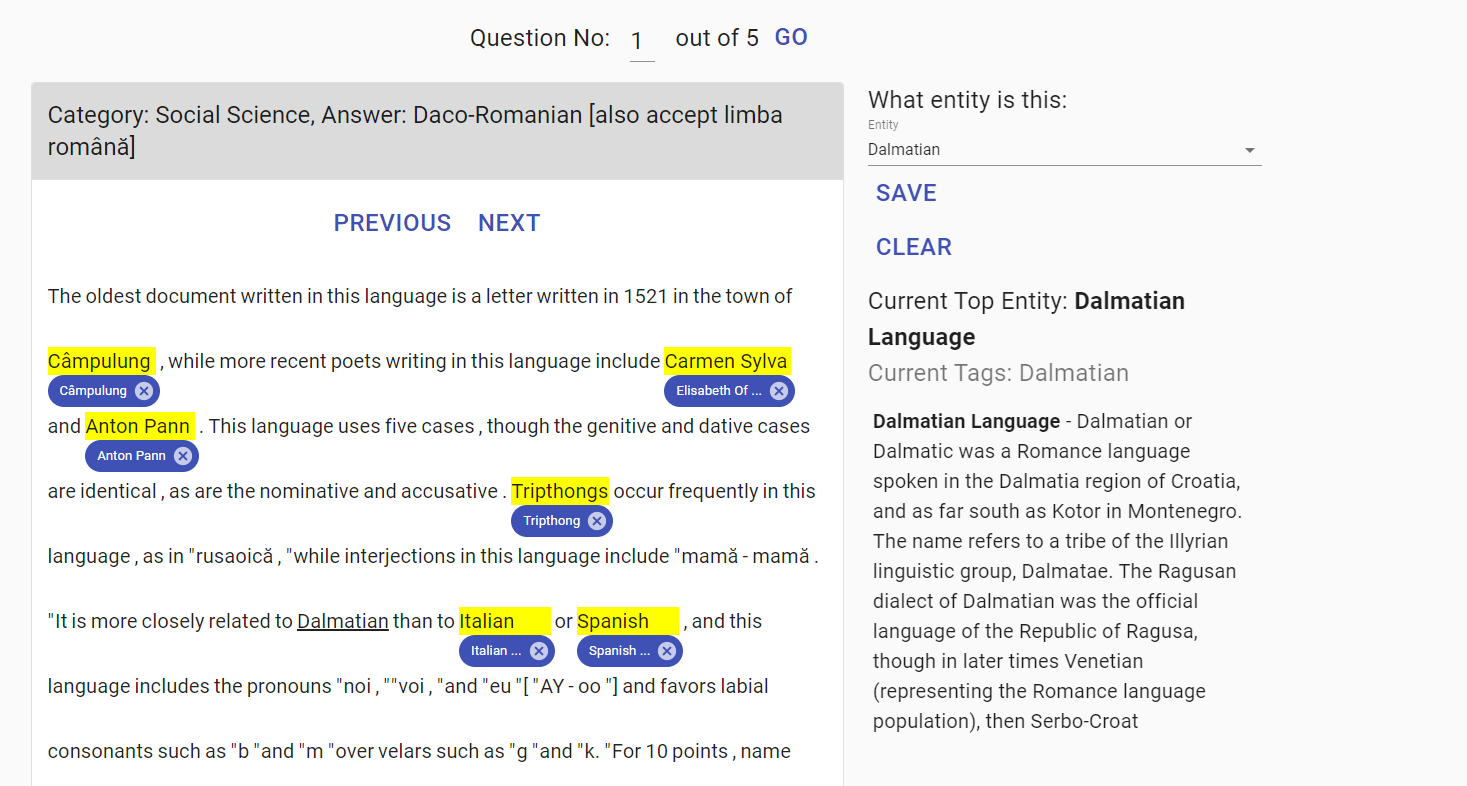
\includegraphics[width=\columnwidth]{quel-interface}
    \caption{
        We show our annotation interface currently, which has the ability to select text spans and tag them with an entity. 
        We plan to suggest noun phrases to annotate in the future, and also plan to allow users to annotate nested spans. 
    }
    \label{fig:nel-int}
\end{figure}


We plan to add annotations for subspans, otherwise known as nested entities. 
Examples of this include the entity "Washington crossing the Delaware"; the whole entity would be matched with the painting, while Washington would be linked to George Washington and Delaware would be linked to Delaware. 
We propose two methods of doing this
\begin{enumerate}
	\item List of noun phrase suggestions, which includes nested noun phrases. 
	The user simply has to annotate each noun phrase. This would reduce the time needed for annotation, as the user does not need to search for noun phrases. 
	\item Augment the current interface with nested spans, allowing users to tag a particular word or phrase as part of multiple entities. 
	While simpler to implement, this option might be less user friendly. 
\end{enumerate}




\subsection{Using other Entity Linkers}
\label{sec:other-ent} 
We utilize different experimental conditions to speed up the entity linking process by pre-populating entity links. 
Later (Section~\ref{sec:exp}), we propose experiments to compare different experimental conditions to determine which condition would optimize entity linking accuracy and speed. 
Before a question is loaded, we assign the annotator an experimental condition that decides how entity links are pre-populated.
In the first condition, no entity links are pre-populated so the question is annotated from scratch.
The second condition pre-populates entity links with the output of one randomly selected entity linker. 
In the third condition, we use a named entity recognition system to display candidate mentions, but do not pre-link them to Wikipedia entities.
The final condition pre-populates links that are predicted by two or more of the linkers.
Later, we analyze the annotation differences on a shared set of questions as well as distributionally across the non-shared questions.

\subsection{Human-in-the-Loop Annotation}
\label{sec:active} 
Prior research has shown that human-in-the-loop annotation for entity linking tasks can speed up the process~\cite{klie2020hero}. 
To do this, we plan to recommend which entities a particular noun phrase might be linked to via a model, so that  our annotation system assists users with determining what noun phrased are linked to. 
At the moment, we plan to build two simple baseline models. 
The first model recognizes noun phrases based off of n-grams, though we could also use some type of BERT based embedding~\cite{devlin2018bert}. 
The second model uses these noun phrases and links them to a Wikipedia page. 
The model will deliver a confidence score for a list of entities associated with each noun phrase, and we let the user select among these options to assist them with entity linking. 
With this, annotators can focus on annotating lower confidence entities. 
As the model improves, our suggestions will also improve, and annotators will be able to annotate faster. 
We additionally use information from user annotations to determine which noun phrases can be pre-annotated, saving annotators time in finding noun phrases.


\subsection{Gold Annotations}
\label{sec:gold}
Prior to scaling our data collection, we annotated a gold set of ten development set questions in \qb{}; in the future, we plan to annotate one hundred development set questions in \qb{}, \triviaqa{}, and \searchqa{}.
For gold annotation, we---the authors---plan to doubly annotate each question from scratch. 
We plan to iteratively annotate twenty-five questions at a time before checking for annotation disagreements.
On disagreement, we plan to either identify the mistake, identify unclear guidelines, or identify genuinely ambiguous cases.
To create the final gold set, we plan to exclude ambiguous cases and reach a consensus on disagreements.
To determine inter-rater reliability, we plan to use kappa scores~\cite{mchugh2012interrater}.  


\subsection{Motivating Experts to Annotate}
\label{sec:packet}
Instead of crowd workers, we work with the \qb{} community, where incentives are aligned. 
Within this community, it is valuable for players to know the distribution of topics and entities to help them study. 
It is similarly helpful for question writers to know the distribution of question topics so that they can design tournaments with a diverse collection of entities. 
To support the \qb{} community, we plan to build two features.
First, we plan to add a \emph{tournament view} that aggregates information from all questions in a tournament, such as the distribution of topics, which entities were mentioned, and the types of entities mentioned.
This allows tournament organizers to know which entities are under and over-represented when writing questions. 
Second, we plan to build an interface where users can search for questions based on the entities mentioned, types of the entities, and topic area.
This allows users to study based on particular entities, and find out the context that a particular entity appears in. 
Using expert trivia competitors instead of crowd workers is better, due to the skill level of these competitors. 
Their annotations would accurately identify entities, and annotate them, allowing for a higher quality dataset, that is also annotated faster. 

\subsection{Quality Control}
\label{sec:expert}
In addition to aligning incentives, we also plan to control annotation quality through multiple annotations and test examples.
We only plan to use questions that were annotated at least twice, and we measure inter-annotator agreement using kappa scores~\cite{mchugh2012interrater}.
Additionally, we plan to annotate two questions per packet, which we use as canaries to detect under-performing annotators.
If the same user annotates too many canaries incorrectly, we disregard all their annotations.


